\documentclass{standalone}
\usepackage[svgnames]{xcolor} % Enables a wide range of color names
\usepackage{tikz}
\usetikzlibrary{arrows,automata,positioning,shapes}
\usepackage{amsmath,amssymb,amsfonts}

\begin{document}
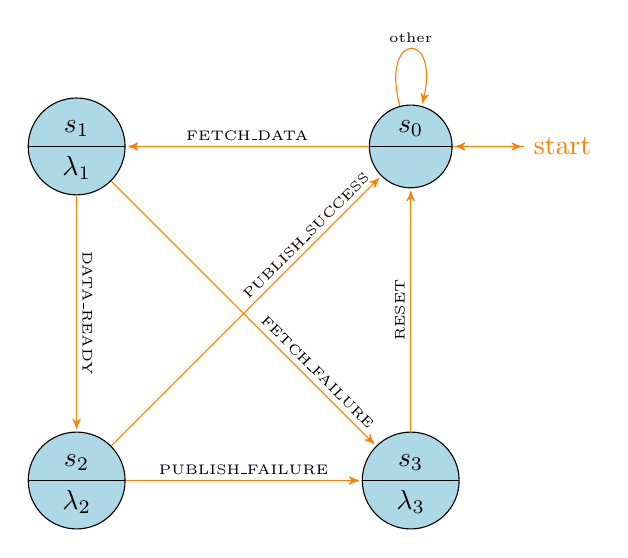
\begin{tikzpicture}[
                    scale=2,
                    >=stealth',
                    shorten > = 1pt,
                    node distance = 1cm and 2cm,
                    el/.style = {inner sep=2pt, align=left, sloped, color=black, font=\tiny},
                    every label/.append style = {font=\tiny},
                    every node/.append style ={font=\normalsize},
                    every state/.append style={fill=LightBlue},
                    every edge/.append style={color=orange},
                    state/.style=state with output,
                    accepting/.style=accepting by arrow,
                    square/.style={regular polygon, regular polygon sides=4, minimum size=6cm, outer sep=0pt}
                    ]
\tikzset{
  sigma_1/.style={node contents=FETCH\_DATA},
  sigma_2/.style={node contents=DATA\_READY},
  sigma_3/.style={node contents=FETCH\_FAILURE},
  sigma_4/.style={node contents=PUBLISH\_SUCCESS},
  sigma_5/.style={node contents=PUBLISH\_FAILURE},
  sigma_6/.style={node contents=RESET}
}

\node[square] (A) {};

\node[state,accepting,
      initial right] (q0) at (A.corner 1) {$s_0$};
\node[state]         (q1) at (A.corner 2) {$s_1$\nodepart{lower} $\lambda_1$};
\node[state]         (q2) at (A.corner 3) {$s_2$\nodepart{lower} $\lambda_2$};
\node[state]         (q3) at (A.corner 4) {$s_3$\nodepart{lower} $\lambda_3$};

\path[->]
    (q0) edge [loop above] node[el] {other}        (q0)
    (q0)  edge  node[el,above,sigma_1] {}          (q1)
    (q1)  edge  node[el,above,sigma_2] {}          (q2)
    (q1)  edge  node[el,above,pos=0.75,sigma_3] {} (q3)
    (q2)  edge  node[el,above,pos=0.75,sigma_4] {} (q0)
    (q2)  edge  node[el,above,sigma_5]  {}         (q3)
    (q3)  edge  node[el,above,sigma_6]  {}         (q0);
\end{tikzpicture}
\end{document}